\chapter{Επιλογές και Προτάσεις}
\section{Κριτήρια Αξιολόγησης Επιλογών}
Λαμβάνοντας υπόψιν τις λειτουργικές και μη λειτουργικές απαιτήσεις του συστήματος που αναλύθηκαν στις ενότητες \ref{3.1} και \ref{3.2},
προέκυψαν τα παρακάτω μετρήσιμα κριτήρια ώστε να μπορεί ο πελάτης να συγκρίνει τις διαθέσιμες επιλογές του και να προβεί στην καλύτερη 
δυνατή λύση. Ειδικότερα, τα κριτήρια αυτά είναι:
\begin{enumerate}
	\item Ταχεία και εύκολη εξυπηρέτηση των πελατών
	\item  Φιλικό γραφικό περιβάλλον τόσο για τους πελάτες αλλά και το προσωπικό
	\item  Χρόνος εκμάθησης για το προσωπικό
	\item Απρόσκοπτη πρόσβαση καθ’ όλη την διάρκεια της ημέρας
	\item Βέλτιστη αξιοποίηση προσωπικού της επιχείρησης
	\item Χρόνος ανάπτυξης
	\item Χρόνος εγκατάστασης
	\item Κόστος ανάπτυξης
	\item Κόστος εγκατάστασης
	\item Κόστος συντήρησης
	\item Περιθώριο αύξησης του κέρδους
	\item Ασφάλεια συστήματος τόσο από κυβερνοεπιθέσεις αλλά και από φυσικά φαινόμενα
\end{enumerate}

\section{Εμπορικά Πακέτα Λογισμικού}
\subsection{Ανάλυση πακέτου Suitepad}
\subsubsection{Περιγραφή πακέτου}
Το εμπορικό πακέτο Suitepad της Suitepad GmbH καλύπτει το ένα μέρος του συστήματος 
που επιθυμεί ο πελάτης. Αναλυτικότερα, όλες οι ιδέες του πελάτης για την χρήση των 
τάμπλετ στα δωμάτια υλοποιούνται από το πακέτο. Προσφέρει καλύτερη επικοινωνία με 
τη reception μέσω του digital guest directory που παρέχει, ενώ παράλληλα ενημερώνει τον 
πελάτη για το τι μπορεί να παραγγείλει με room-service. Άλλη χρήσιμη λειτουργία που 
προσφέρει είναι το Suitepad lobby screen, ένας τρόπος να διαφημίζει το ξενοδοχείο τοπικές 
δραστηριότητες και συνεργαζόμενα μαγαζιά και εστιατόρια για να απασχολήσει τον πελάτη 
κατά τη διαμονή του και να αφήσει σε αυτόν μια καλύτερη εντύπωση. Επιπλέον δυνατότητα 
είναι το Suitepad BYOD (bring your own device), που δίνει στους πελάτες όλες τις υπόλοιπες 
λειτουργίες του πακέτου όταν δε βρίσκονται στο δωμάτιο, με την παροχή ενός personalized 
link, δηλαδή μίας ιστοσελίδας για το ξενοδοχείο που οι πελάτες θα μπορούν να σώζουν στο 
κινητό τους και να τη χρησιμοποιούν κατά τη διαμονή τους. 

\clearpage 
\noindent
Κάποιες τελευταίες λειτουργίες  του πακέτου είναι το Suitepad phone, που αντικαθιστά τα 
τηλέφωνα για τον τρόπο επικοινωνίας μεταξύ δωματίων καθώς και το Suitepad TV control 
και Suitecast, που μετατρέπουν την τηλεόραση του δωματίου σε ένα σύγχρονο μέσο 
ψυχαγωγίας (ώστε ο χρήστης να μπορεί να συνδεθεί με πλατφόρμες όπως Netflix, amazon 
prime, Spotify). Η τιμή αυτού του πακέτου καθορίζεται με βάση το μέγεθος του ξενοδοχείου 
μετά από επικοινωνία με την εταιρία, αλλά έχουμε βρει πως για μικρότερες επιχειρήσεις το 
κόστος εγκατάστασης τείνει στα 880 ευρώ για την εγκατάσταση, ενώ στη συνέχεια έχει ένα 
μηνιαίο κόστος 55 ευρώ. Παρότι η τιμή του μπορεί να θεωρηθεί καλή, αξίζει να αναφερθεί 
πως αποτελεί ρίσκο, ειδικά για ένα καινούριο ξενοδοχείο και πρέπει να γίνει υπολογισμός 
εάν το συμφέρει η επένδυση. Είναι σημαντικό να αναφερθεί ακόμα ότι με το Suitepad δεν 
καλύπτεται η ανάγκη που εξέφρασε ο πελάτης για καλύτερη καταγραφή των προμηθειών 
που χρειάζονται. \\

\subsubsection{Ανάλυση Σκοπιμότητας}
Όπως ενημερωθήκαμε από την γραμματεία το υπάρχον πρόγραμμα δεν εξυπηρετεί καλά το 
προσωπικό και ξοδεύουν πολύ περισσότερο χρόνο από τι χρειάζεται για να συμπληρώσουν 
τι χρειάζονται να προμηθευτούν. Το Suitepad, έχει μια ικανοποιητική πλατφόρμα για την 
καταγραφή προϊόντων που χρειάζονται και πρόκειται για ένα σύστημα που θα είναι εύκολα 
κατανοητό από το προσωπικό. Συμπληρωματικά, προσφέρει έναν τρόπο επικοινωνίας 
μεταξύ του φιλοξενούμενου και του προσωπικού το οποίο ήταν το άλλο σημαντικό αίτημα 
του πελάτη καθώς έτσι θα αφήνουν καλύτερες εντυπώσεις και θα αυξάνουν τις πιθανότητες 
ο φιλοξενούμενος να επιστρέψει σε μελλοντική σεζόν. Τέλος, το συγκεκριμένο εμπορικό 
πακέτο εκπληρώνει και το αίτημα του πελάτη για την αξιοποίηση των ήδη υπάρχοντων 
τάμπλετ στα δωμάτια για την ψυχαγωγία του φιλοξενούμενου. \\

\subsubsection{Τεχνική Σκοπιμότητα}
Η απαραίτητη τεχνολογία για την υλοποίηση των λειτουργιών που θέλουμε να 
πραγματοποιήσουμε είναι άμεσα διαθέσιμη. Η χρήση της δεν είναι εύκολη και 
αναφερόμαστε για ένα  project το οποίο θα ολοκληρωθεί σε βάθος χρόνου (2-3 μήνες)
αλλά δεδομένου της μακροχρόνιας παρουσίας της στον εν λόγω χώρο, αποπνέει έναν αέρα 
ασφάλειας και την κρίνει μια σαφώς κατάλληλη αλλά και ορθολογική επιλογή. Η άρτια 
καταρτισμένη μας ομάδα θα αξιοποιήσει τις γνώσεις και τους απαιτούμενους πόρους με 
σκοπό να φέρει εις πέρας το έργο αυτό. Σκοπός μας μεταξύ άλλων είναι να εμπνεύσουμε την 
ασφάλεια που χρειάζεται η επιχείρηση για να πλεύσει σε άγνωστα για αυτήν νερά, και 
μπορούμε με βεβαιότητα να πούμε ότι η τελική παράδοση του εν λόγω project θα αφήσει 
και τις δύο μεριές της παρούσας συνεργασίας ικανοποιημένες. \\

\subsubsection{Ανάλυση χρονοδιαγράμματος}
Σαφώς, η ύπαρξη ενός νέου προγράμματος και η εκμάθηση του θα είναι μια διαδικασία η 
οποία χρειάζεται χρόνο. Ωστόσο δεν παρουσιάζει σημαντικές τεχνικές δυσκολίες αλλά 
ούτε και χρειάζονται προαπαιτούμενες γνώσεις πέραν της χρήσης Η/Υ. Ο χρόνος 
εκμάθησης εκτιμάται περίπου στη μία βδομάδα για κάθε υπάλληλο.Το πρόβλημα που 
παρουσιάζεται είναι η έλλειψη χρόνου των εργαζομένων σε περιόδους ανόδου της 
δουλειάς και λόγω φόρτου εργασίας να είναι δύσκολο να αφιερωθούν οι απαραίτητες 
ώρες για την εκμάθηση του. Υπολογίζουμε όμως ως ομάδα ανάπτυξης του παρόντος 
πακέτου, πώς κατά την χρήση του από επιχειρήσεις θα είμαστε σε κάθε βήμα εκμάθησής 
του δίπλα τους με σκοπό την ομαλότερη και καλύτερη εκπαίδευσης τους.  
\clearpage  

\subsubsection{Οικονομική Ανάλυση}
\textbf{Ανάλυση Κόστους (Cost Analysis)}: Όπως αναφέρθηκε πιο πάνω το εμπορικό 
πακέτο Suitepad έχει ένα κόστος εγκατάστασης, που είναι ανεξάρτητο από το μέγεθος 
του ξενοδοχείου, και ανέρχεται στα 1000 ευρώ. Πέρα από αυτή την αρχική χρέωση, 
μπορούμε να θεωρήσουμε ότι λόγω του μεγέθους του ξενοδοχείου θα πληρώνουν γύρω 
στα 60 ευρώ το μήνα. Στο κοντινό μέλλον (μετά από 3 χρόνια) μπορούμε να θεωρήσουμε 
ότι το ξενοδοχείο θα έχει περισσότερα δωμάτια και η μηνιαία συνδρομή μπορεί να ανέρθει 
στα 70 ευρώ το μήνα. Τέλος, παρότι το πακέτο χαρακτηρίζεται απλοϊκό για τους χρήστες, 
πρέπει να θεωρήσουμε ότι το προσωπικό θα χρειάζεται ένα χρονικό διάστημα για να 
εκπαιδευτεί στο πως να το χειρίζεται, τον χαμένο αυτό χρόνο τον έχω μεταφράσει ως μία 
εβδομάδα κάθε εξάμηνο για κάθε εργαζόμενο (σε περίπτωση που υπάρξουν updates απ' 
τους δημιουργούς).

% Please add the following required packages to your document preamble:
% \usepackage{graphicx}
\begin{table}[H]
	\resizebox{\textwidth}{!}{%
		\begin{tabular}{|c|c|c|c|c|c|c|}
			\hline
			Year            & 0     & 1     & 2     & 3     & 4     & 5     \\ \hline
			one-time costs  & 1000  & -     & -     & -     & -     & -     \\ \hline
			Recursive costs & 2.945€ & 2.945€ & 2.945€ & 3.065€ & 3.065€ & 3.065€ \\ \hline
		\end{tabular}%
	}
\end{table}

\noindent
\\ \textbf{Ανάλυση Οφέλους (Benefit Analysis)}: Βασικό πλεονέκτημα που θα προσφέρει 
αυτό το εμπορικό πακέτο είναι η εξοικονόμηση χρόνου για όλο το προσωπικό, καθώς 
θα βελτιώσει και θα κάνει πιο εύκολη την επικοινωνία μεταξύ τους. Μετά από ένα χρονικό 
διάστημα, ελπίζουμε οι καλές εντυπώσεις που θα έχει αφήσει η επικοινωνία μεταξύ του 
προσωπικού και των πελατών, να κάνει κάποιους πελάτες να επιστρέψουν, που θα 
μεταφράζεται σαν μια μικρή αύξηση στις σεζόν που δεν υπάρχει πολύ ενασχόληση.

% Please add the following required packages to your document preamble:
% \usepackage{graphicx}
\begin{table}[H]
	\centering
	\resizebox{\textwidth}{!}{%
		\begin{tabular}{|c|c|c|c|c|c|c|}
			\hline
			Year     & 0     & 1     & 2     & 3     & 4     & 5     \\ \hline
			Benefits & 2.848€ & 3.132€ & 3.627€ & 3.913€ & 4.199€ & 4.816€ \\ \hline
		\end{tabular}%
	}
\end{table}

\subsubsection{Ανάλυση Απόσβεσης (Payback Analysis)}
\begin{table}[H]
	\begin{tabular}{|c|c|}
		\hline
		Κέρδος                        & Έτος \\ \hline
		{\color[HTML]{FE0000} -1.097€} & 0    \\ \hline
		{\color[HTML]{FE0000} -917€} & 1    \\ \hline
		{\color[HTML]{FE0000} -287€} & 2    \\ \hline
		467€                           & 3    \\ \hline
		1.436€                         & 4    \\ \hline
		2.875 €                       & 5    \\ \hline
	\end{tabular}
\end{table}

\begin{figure}[H]
	\centering
	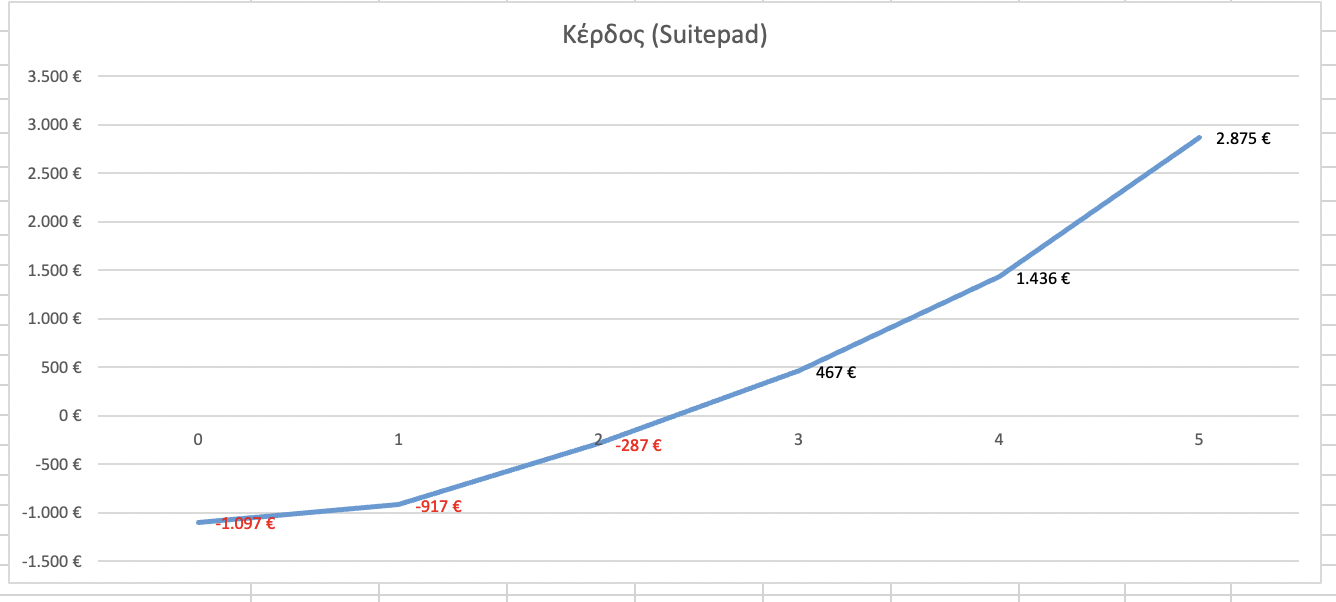
\includegraphics[width=1\textwidth]{Images/4.2.2}
\end{figure}

\noindent
Αν κάνουμε τη διαίρεση που υπάρχει στη θεωρία θα δούμε ότι η απόσβεση γίνεται στα 
3.38 έτη (με το 0 να μετράει σαν το πρώτο έτος). \\ \\

\subsubsection{Διάγραμμα ROI (Return on Investment)}
\begin{figure}[H]
	\centering
	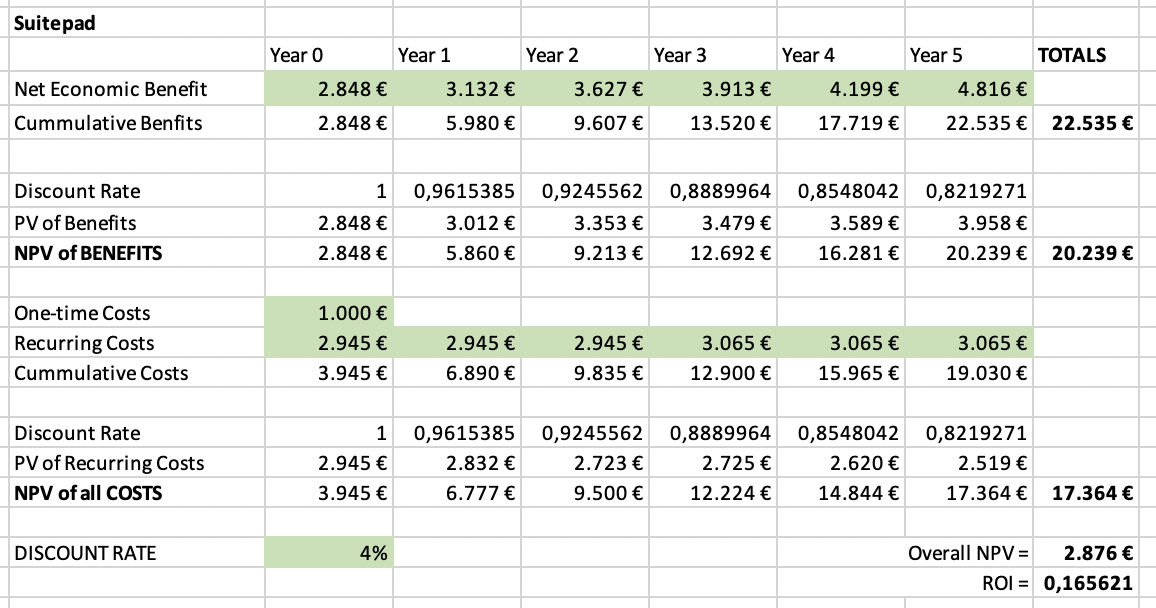
\includegraphics[width=1\textwidth]{Images/4.2.3}
\end{figure}
\clearpage

\subsection{Ανάλυση πακέτου Mini Hotel}
\subsubsection{Ανάλυση Σκοπιμότητας}
Καθώς δεν υπάρχει παρών σύστημα το οποίο να ικανοποιεί έστω σε έναν βαθμό τις 
απαιτήσεις του πελάτη μας, είναι απαραίτητη η ύπαρξη ενός πακέτου που θα 
περιλαμβάνει χαρακτηριστικά απαραίτητα για την ομαλή διεκπεραίωση των 
διεργασιών της επιχείρησης καταλυμάτων \textbf{Balance Hotel Chania}. Η υπεύθυνη 
που έχει ορίσει ο πελάτης μας για την διεύθυνση της λειτουργίας της επιχείρησης έχει 
τις απαραίτητες γνώσεις για να κατανοήσει και να αξιοποιήσει το εκάστοτε πρόγραμμα, 
καθώς και την αμέριστη τεχνική υποστήριξη της ομάδας για οποιαδήποτε μελλοντική 
απορία/ δυσχέρεια παρουσιαστεί. Έχει ήδη επιβεβαιωθεί από την ίδια και κυριότερα 
από τον ιδιοκτήτη ότι η προσθήκη αυτή του συστήματος θα είναι ευνοϊκή για την ομαλή 
λειτουργία της επιχείρησης. Από νομική σκοπιά υπάρχει επίσης κάλυψη.

\subsubsection{Σκοπιμότητα Χρονοδιαγράμματος}
Η προσθήκη ενός νέου προγράμματος σαφώς και θα απαιτεί κάποιες βασικές διαδικασίες .
Αρχικά, είναι απαραίτητη η εγκατάσταση τεχνικών υποδομών για την σωστή λειτουργία 
της εφαρμογής, μία διαδικασία που θα ήταν θεμιτό να έχει ολοκληρωθεί σε μία με δύο 
εργάσιμες. Ακόμα, το νέο σύστημα θα χρησιμοποιείται από τους υπαλλήλους και όπως 
κάθε νέα τεχνολογία, θα απαιτεί κάποιο χρόνο εκμάθησης για τους υπαλλήλους. Θεμιτό 
θα ήταν αυτή η εκπαίδευση να μην υπερβαίνει την μία εβδομάδα για κάθε εργαζόμενο.

\subsubsection{Οικονομική Ανάλυση}
\textbf{Ανάλυση Κόστους}: Όπως αναφέρθηκε πιο πάνω το συγκεκριμένο εμπορικό πακέτο 
δεν έχει κάποιο κόστος εγκατάστασης αλλά έχει μια μηνιαία συνδρομή που ανέρχεται στα 92€. 
Όμως, όπως αναφέρθηκε και στο προηγούμενο εμπορικό πακέτο, η προσαρμογή του 
προσωπικού στον τρόπο λειτουργίας του θα μεταφραστεί σαν μία εβδομάδα κάθε εξάμηνο 
και επειδή ο ιδιοκτήτης μπορεί να θελήσει να  αυξήσει τον αριθμό των δωματίων του 
ξενοδοχείου η μηνιαία συνδρομή θα αυξηθεί.

% Please add the following required packages to your document preamble:
% \usepackage{graphicx}
\begin{table}[H]
	\resizebox{\textwidth}{!}{%
		\begin{tabular}{|c|c|c|c|c|c|c|}
			\hline
			Year            & 0     & 1     & 2     & 3     & 4     & 5     \\ \hline
			one-time costs  & 0     & -     & -     & -     & -     & -     \\ \hline
			Recursive costs & 3.292 €& 3.292€ & 3.292€ & 3.438€ & 3.438€ & 3.438€ \\ \hline
		\end{tabular}%
	}
\end{table}

\noindent
\textbf{Ανάλυση Οφέλους (Benefit Analysis)}: Επειδή οι ιδιότητες που προσφέρει είναι πολύ 
όμοιες με αυτές του εμπορικού πακέτου της Suitepad μπορούμε να θεωρήσουμε ότι οι 
επιδράσεις του απτή πλευρά των εσόδων θα είναι παρόμοια.

% Please add the following required packages to your document preamble:
% \usepackage{graphicx}
\begin{table}[H]
	\resizebox{\textwidth}{!}{%
		\begin{tabular}{|c|c|c|c|c|c|c|}
			\hline
			Year            & 0     & 1     & 2     & 3     & 4     & 5     \\ \hline
			Recursive costs & 2.848€ & 3.132€ & 3.627€ & 3.913€ & 4.199€ & 4.816€ \\ \hline
		\end{tabular}%
	}
\end{table}

\subsubsection{Ανάλυση Απόσβεσης (Payback Analysis)}
% Please add the following required packages to your document preamble:
% \usepackage[table,xcdraw]{xcolor}
% If you use beamer only pass "xcolor=table" option, i.e. \documentclass[xcolor=table]{beamer}
\begin{table}[H]
	\begin{tabular}{|c|c|}
		\hline
		Κέρδος                      & Έτος \\ \hline
		{\color[HTML]{FE0000} -444€} & 0    \\ \hline
		{\color[HTML]{FE0000} -597€} & 1    \\ \hline
		{\color[HTML]{FE0000} -288€} & 2    \\ \hline
		405€                         & 3    \\ \hline
		785€                         & 4    \\ \hline
		1.917€                       & 5    \\ \hline
	\end{tabular}
\end{table}

\begin{figure}[H]
	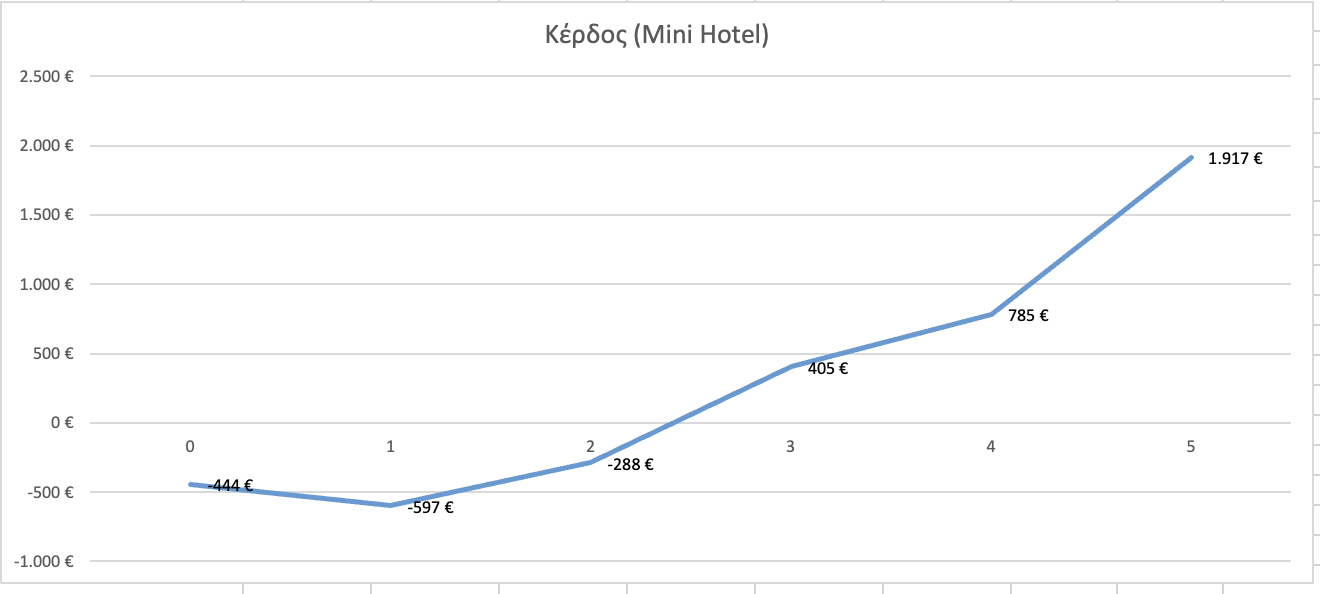
\includegraphics[width=0.8\textwidth]{Images/4.2.5}
\end{figure}

\noindent
Αν κάνουμε τη διαίρεση που υπάρχει στη θεωρία θα δούμε ότι η απόσβεση γίνεται στα 
3.41 έτη (με το 0 να μετράει σαν το πρώτο έτος).

\subsubsection{Διάγραμμα ROI (Return on Investment)}
\begin{figure}[H]
	\centering
	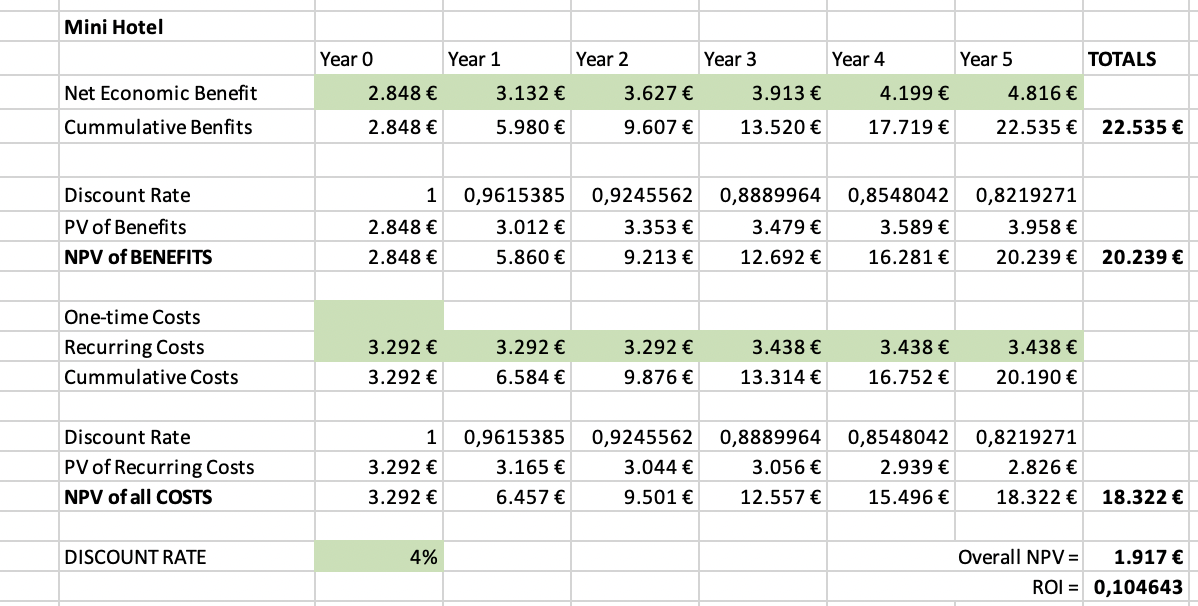
\includegraphics[width=1\textwidth]{Images/4.2.6}
\end{figure}

\section{Επιλογή Ανάπτυξης Νέου Συστήματος}
\subsubsection{Περιγραφή Πακέτου}
Το εμπορικό πακέτο που προετοιμάζουμε μοιάζει με τα προηγούμενα στα περισσότερα 
χαρακτηριστικά αλλά επιλέξαμε να κάνουμε το καλύτερο δυνατό των δύο κόσμων: να 
δημιουργήσουμε ένα πακέτο σε χαμηλότερη τιμή από το 1ο εμπορικό πακέτο, ενώ 
παράλληλα να καταφέρουμε να αφομοιώσουμε την διεργασία της ενδοεπικοινωνίας 
μεταξύ πελάτη και προσωπικού που προσφέρει το 1ο εμπορικό πακέτο της \textbf{
Suitepad GmbH} αλλά λείπει από το αντίστοιχο της \textbf{Mini Hotel PMS}. Έτσι 
καταφέρνουμε να είμαστε οικονομικά προσιτοί σε μικρότερες οικογενειακές επιχειρήσεις,
προσφέροντας παράλληλα υπηρεσίες οι οποίες δύσκολα απαντώνται σε άλλα εξίσου 
χαμηλού κόστους πακέτα. \\

\noindent
Στα πλεονεκτήματα αναφέρουμε την καθαρή και around the clock επικοινωνία πελάτη με 
την υποδοχή ή την υπεύθυνη μέσω κατάλληλου interface ώστε να αποφεύγεται η 
ενόχληση των εργαζομένων σε προγράμματα όπως το Viber ή το Whatsapp και να υπάρχει 
επαγγελματισμός. Επίσης να αναφερθούμε στο ότι υλοποιείται ένα FAQ ερωτηματολόγιο με 
στάνταρ ερωτήσεις για τους πελάτες της επιχείρησης οι οποίες μπορούν να αλλάζουν την 
κάθε περίοδο κατόπιν έρευνας στις ανάγκες των πελατών. Επίσης η δυνατότητα για 
housekeeping είναι μία από αυτές που προσφέρονται στο πακέτο μας και μας έχει ήδη 
γνωστοποιηθεί από τον υπεύθυνο ότι είναι μια λειτουργία που του χρειάζεται. Σημαντικό 
ακόμα πλεονέκτημα είναι το ότι προσφέρουμε την δυνατότητα μέσω νέου UI στον πελάτη 
να μπορεί να παραγγείλει στην υποδοχή ποτό, κρασί ή αφέψημα καθώς και ολοκληρωμένο 
γεύμα (πρωινό, βραδινό) αλλά και να επιλέξει ο ίδιος την ώρα παράδοσής του με δύο κλικ 
μέσα από τον υπάρχοντα κατάλογο της κάβας/μενού της επιχείρησης. \\

\noindent
Ένα μειονέκτημα του υπό ανάπτυξη πακέτου είναι ότι δεν έχουμε αξιοποιήσει τα tablet που 
παρέχει η επιχείρηση με σκοπό και την ρύθμιση των smart home συσκευών του εκάστοτε 
δωματίου του καταλύματος.Ακόμα αναγνωρίζουμε πώς λόγω του ότι το πακέτο δεν είναι 
ακόμα διαθέσιμο, ίσως ο αγοραστής μας να αποχωρήσει καθώς χρειάζεται σύντομα την 
ύπαρξη ενός πληροφοριακού συστήματος για την καλύτερη εξυπηρέτηση των αναγκών του.

\subsubsection{Ανάλυση Χρονοδιαγράμματος}
Για την δικιά μας εφαρμογή σημαντικός στόχος ως προς τον χρόνο θα ήταν η ολοκλήρωση 
σχεδόν όλων των βασικών διεργασιών προς το τέλος του πρώτου μήνα, έτσι ώστε η ομάδα 
του software-engineering να τελειώνει με την εφαρμογή προς το τέλος του δεύτερου μήνα για 
να αποφύγουμε τη μισθοδοσία του τρίτου. Το άλλο σημαντικό κομμάτι θα είναι η εκπαίδευση 
του προσωπικού, η οποία έχουμε σαν στόχο να έχει ολοκληρωθεί μέσα στο πλαίσιο μιας 
εργάσιμης εβδομάδας.

\subsubsection{Οικονομική Ανάλυση}
\textbf{Ανάλυση Κόστους (Cost Analysis)}: Το κύριο κόστος της εφαρμογής μας βγαίνει από 
την κατασκευή του, η οποία θα γίνει από ένα software engineering team και θα διαρκέσει 
2-3 μήνες. Αυτή η διαδικασία θα κοστίσει περίπου 2120€ και όπως και στα εμπορικά πακέτα 
θα θεωρήσουμε πως θα κοστίσει στο ξενοδοχείο μια εβδομάδα εργασίας του προσωπικού, 
όμως η συχνότητα εκπαίδευσης θα είναι διαφορετική. Συγκεκριμένα, αν θεωρήσουμε ότι το 
ξενοδοχείο χρειάζεται να αναβαθμίσει την εφαρμογή κάθε 3 χρόνια τότε το προσωπικό θα 
χρειάζεται να ξαναεκπαιδευτεί σε αυτές τις περιπτώσεις. (Για την αναβάθμιση θα θεωρήσουμε 
ότι χρησιμοποιούμε την ίδια ομάδα software-engineering για ένα χρονικό διάστημα ενός μήνα)

% Please add the following required packages to your document preamble:
% \usepackage{graphicx}
\begin{table}[H]
	\resizebox{\textwidth}{!}{%
		\begin{tabular}{|c|c|c|c|c|c|c|}
			\hline
			Year            & 0     & 1 & 2     & 3 & 4     & 5 \\ \hline
			one-time costs  & 3.233€  & - & 2.010€  & - & 1.858€   & - \\ \hline
			Recursive costs & -     & - & -     & - & -     & - \\ \hline
		\end{tabular}%
	}
\end{table}

\noindent
\textbf{Ανάλυση Οφέλους (Benefit Analysis)}: Καθώς η εφαρμογή δεν προσφέρει επιπλέον 
ψυχαγωγία στον φιλοξενούμενο μπορούμε να θεωρήσουμε πως ο ρυθμός αύξησης σε πελάτες 
που επισκέπτονται σε σεζόν λίγης απασχόλησης, από τον τρίτο χρόνο και μετά θα είναι  
χαμηλότερος.

% Please add the following required packages to your document preamble:
% \usepackage{graphicx}
\begin{table}[H]
	\resizebox{\textwidth}{!}{%
		\begin{tabular}{|c|c|c|c|c|c|c|}
			\hline
			Year     & 0     & 1     & 2     & 3     & 4     & 5     \\ \hline
			Benefits & 2.848€  & 3.132€  & 3.627€  & 3.835€  & 2.904€  & 4.247€  \\ \hline
		\end{tabular}%
	}
\end{table}

\subsubsection{Ανάλυση Απόσβεσης (Payback Analysis)}
% Please add the following required packages to your document preamble:
% \usepackage[table,xcdraw]{xcolor}
% If you use beamer only pass "xcolor=table" option, i.e. \documentclass[xcolor=table]{beamer}
\begin{table}[H]
	\begin{tabular}{|c|c|}
		\hline
		Κέρδος                       & Έτος \\ \hline
		{\color[HTML]{FE0000} -385€} & 0    \\ \hline
		2.627€                       & 1    \\ \hline
		3.806€                       & 2    \\ \hline
		7.125€                       & 3    \\ \hline
		8.694€                       & 4    \\ \hline
		12.185€                      & 5    \\ \hline
	\end{tabular}
\end{table}

\begin{figure}[H]
	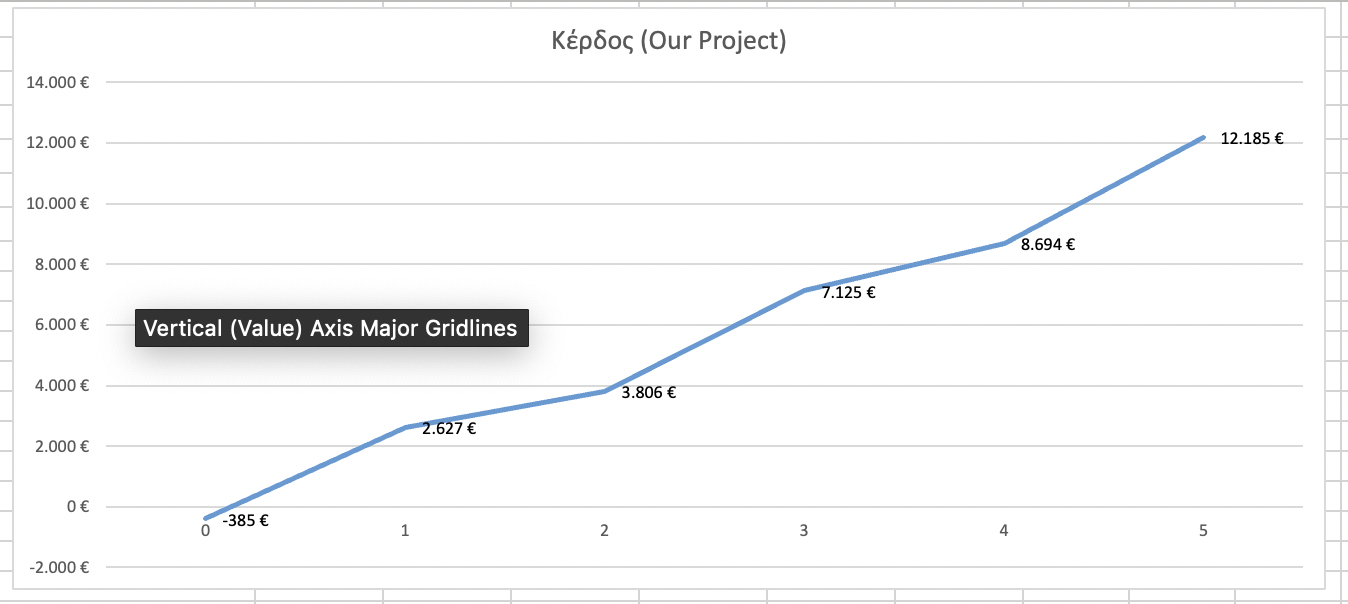
\includegraphics[width=1\textwidth]{Images/4.2.8}
\end{figure}

\noindent
Αν κάνουμε τη διαίρεση που υπάρχει στη θεωρία θα δούμε ότι η απόσβεση 
γίνεται στα 1.13 έτη (με το 0 να μετράει σαν το πρώτο έτος).

\subsubsection{Διάγραμμα ROI (Return on Investment)}
\begin{figure}[H]
	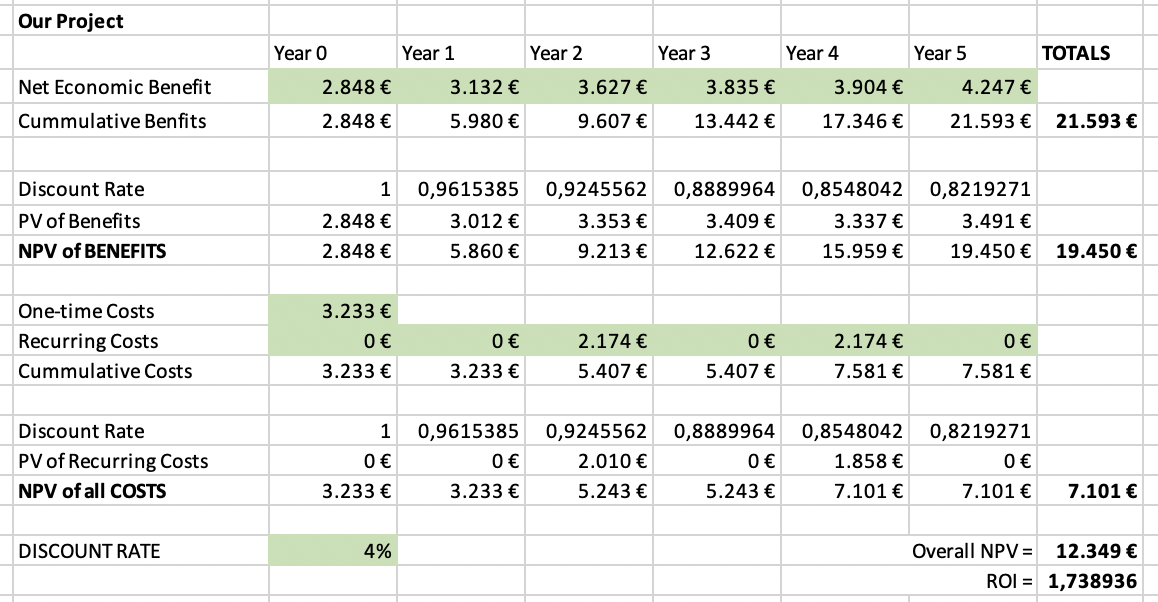
\includegraphics[width=1\textwidth]{Images/4.2.9}
\end{figure}

\section{Τελική Πρόταση}
Λαμβάνοντας υπόψη την οικονομική ανάπτυξη του παραπάνω ερωτήματος καταλήξαμε 
στην απόφαση να προτείνουμε το δικό μας πακέτο στον πελάτη, καθώς επιφέρει τον 
καλύτερο δείκτη ROI. Επιπλέον, πιστεύουμε πως το πακέτο μας καλύπτει σε πολύ 
ικανοποιητικό βαθμό τις απαιτήσεις του πελάτη, αφού δημιουργούμε την πλατφόρμα 
για καλύτερη καταγραφή των προμηθειών και για επικοινωνία του προσωπικού με τον 
φιλοξενούμενο.  
